
\chapter{Introduction}

The Concise Oxford Dictionary of Mathematics defines an anomaly as an unusual and possibly erroneous observation that does not follow the general pattern of a drawn population \cite{Clapham:2013}. Anomaly detection is a branch of data mining that seeks to find data points or patterns that do not fit the overall pattern of the data. Studying anomalous behavior has been applied in many branches of science. For example, an anomalous pattern in financial transaction data could be indicative of fraudulent activity or a an anomalous MRI image may indicate the presence of malignant tumors \cite{Spence:2001:DSC:882464.882797}. Anomaly detection's practicability relies heavily on the simple statistical assumption that rare observations may carry critical information \cite{Chandola:2009:ADS:1541880.1541882}. Detection of an anomaly can have a measurable positive effect and bring far reaching benefits. In the following work I will present anomaly detection using data mining methods on a data set containing credit application forms. The application forms have been submitted via a web interface and include mostly rudimentary personal- as well as financial-information. To collect more information about the credit applicant, the system also tracked technical metrics such as used web-browser and screen resolution. A detailed description of input data will be introduced in the second chapter of this thesis.


\section{Types of Anomalies}

In the context of anomaly detection, anomalies are divided into three categories:

\begin{itemize}
    \item \textit{Point} is the simplest type of an anomaly, it describes an outlier of a single data instance with respect to other data \cite{Chandola:2009:ADS:1541880.1541882}. Given a measurement in several dimensions the point anomaly only affect one of the dimensions. A real world example in financial context can be as follows: Our system predicts anomalies in credit applicant data, one of the data instances is the applicants salary. A salary that is extreme high with respect to the rest of data is a point anomaly.

    \item \textit{Context} is a extension of a point anomaly. A context anomaly describes a possible outlier with respect to it's context. Given a measurement in several dimensions we find that one dimension is anomalous with respect to a different dimension of the same measure. In context anomalies a outlier can only appear in the context of all involved data points and only then \cite{Chandola:2009:ADS:1541880.1541882}. A example from real world can be a credit applicant system described above. Let us assume that we have one one applications with an extreme high salary, if we predict solely based on salary then the application may be indicated anomalous. However, adding the country as another data instance, our model could detect that with respect to the context of country the given salary is not anomalous.

    \item \textit{Collective} anomalies can be detected by observing a collection of relative data points in a data set. Individual data points from the observed collection or sub sequences my not anomalies by themselves, but occurred together they are anomalous \cite{Chandola:2009:ADS:1541880.1541882}. Imagine a credit applicant with following data instances: salary, country, amount applied for. For the sake of simplicity we assume that the credit amount applied for is lower then the salary. Such low application amount is not an anomaly by himself, but in composition with the salary and the country it could be identified as an anomalous pattern for fraudulent behavior. This kind of anomalies have been explored for sequential data \cite{Warrender99detectingintrusion}. This thesis will only treat anomalies in non-sequential data and thus collective anomalies will not be discussed any further.
    
\end{itemize}

\section{Challenges}
Determining whether an observation is an anomaly or a normal observation is closely tied to the questions: what is the general pattern of the data and what is normal according to that pattern? Finding the general pattern of data is subject of active research in statistics, machine learning and artificial intelligence. Drawing a clear line between these fields is irrelevant as many practical methods are a composition rather than a disjunction. This Thesis will treat a machine learning centered approach. A straight forward approach to determine the general pattern of underlying data is creating and training a prediction model. Taking this approach I will have to deal with the following challenges.


\begin{itemize}
    \item Availability of data which label significant anomalous patterns is a common problem in anomaly detection topic. Rare cases are by definition less common in sample data \cite{Weiss:2004:MRU:1007730.1007734}. Identifying them by hand requires domain knowledge and sometimes impossible due to the fact that they haven't occurred yet.
    
    \item Anomalous pattern are not static and can evolve over time. A pattern that is anomalous at a given point in time must not be anomalous in the future and vice versa \cite{Chandola:2009:ADS:1541880.1541882}.
    
    \item To establish the \textit{ground-truth} about anomalous data we need to be provided with sufficient data. Rarity makes result evaluation to a significant problem, in other words with non availability of labeled data, we do not have the base case to compare with \cite{Aggarwal:2013}. %seite 33
    
    \item Distinguishing between noise and anomalies in data leads to a high false positive rate \cite{Chandola:2009:ADS:1541880.1541882}.   % noise in glossary, false positive in glossary
    
\end{itemize}

\section{Machine Learning} 

Deciding on the right machine learning technique to detect anomalies is highly dependant on the model purpose as well as available data. The best choice of a model requires a deep domain knowledge and analysis of available data \cite{Aggarwal:2013}. The relevant data for the described analysis is high dimensional data that contains a small set of positive labeled examples. This observation leads to the fact that we should only consider \textit{semi-supervised} and \textit{unsupervised} learning methods. Moreover we should consider that anomalies in financial data can be a result of malicious actions that were intented to look like normal data. This indicates that the data is noisy and the application we use should have a stable strategy to deal with noisy data. 
In this chapter I will give a brief introduction in  machine learning methods used for anomaly detection and tradeoff their beneficing for our use case. The methods we decide for will be discussed in detail in the third chapter of this work.

\subsection{Extrema-value analysis}

Is an distribution based technique and is one of the most basic form of outlier detection in 1-dimensional data. The core point of this methodology is to find statistical tails with respect to underlying data distribution \cite{Aggarwal:2013}.

Naturally designed for univariate data, extreme value analysis not suit for our use case with high dimensional input data. Nonetheless we should consider that extreme-value analysis play an important role as a final step in most outlier detection algorithms where in final step the data set is represented as a set of univariate values.

\subsection{Proximity-based methods}

The major idea of proximity-based methods is to pool related data sets to groups or cluster based on available data. Data points that are not been allocated to any groups are mostly the outliers.

\textit{Density} based techniques like the nearest neighbour are vulnerable to noise in high dimensional data. Relative contrast between data points decrease with increasing dimensionality \cite{Hinneburg:2000:NNH:645926.671675}. Considering that our sample data is high dimensional this behavior can increase false-negative rate and is thus negligible. 

\begin{figure}
\centering
    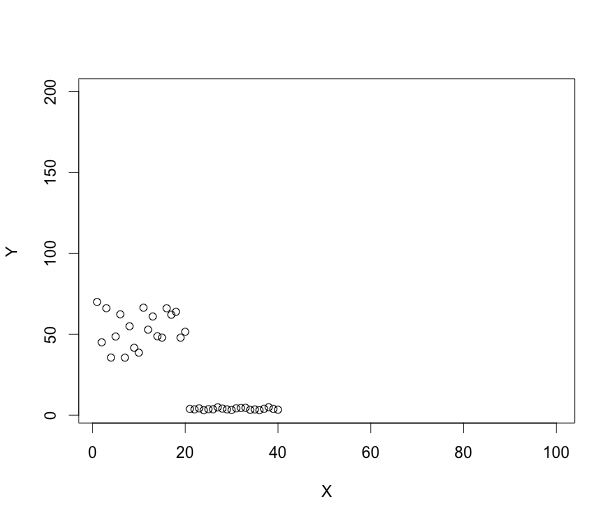
\includegraphics[scale=0.4]{Graphics/plottA.png}
\caption{ X-Y Axis}
 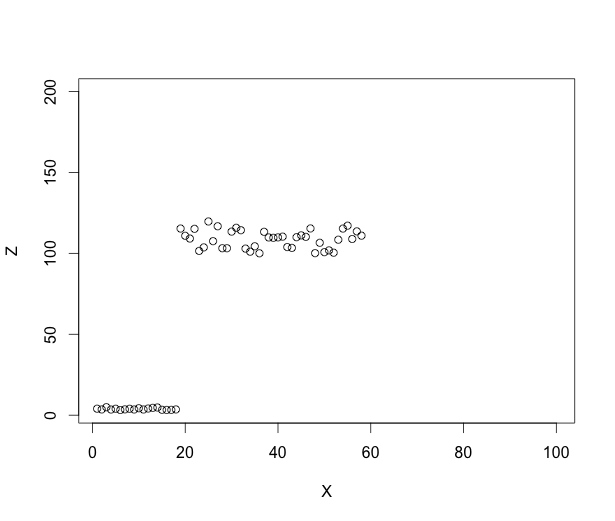
\includegraphics[scale=0.4]{Graphics/plottb.png}
 \caption{ X-Z Axis }
\label{fig:clustering_dimensions}
\end{figure}

\textit{Clustering} algorithms such as the k-means do not work well in high-dimensional space. In  real life in many real data example points are correlating with respect to a given set of dimensions and others with respect to different dimensions \cite{Aggarwal:1999:FAP:304181.304188}. The figure \ref{fig:clustering_dimensions} shows an 3-dimensional space with two patterns, one in \(X\) - \(Y\) plane and another in \(X\) - \(Z\). Clustering in the full dimensional space will not discover the two patterns, since each of them is spread out along one of the dimensions \cite{Aggarwal:1999:FAP:304181.304188}.The weaknesses of proximity-based methods in respect to our use case are the high computation time \(O(2)\) and the fact that anomalies are often lost in the noise when methods are applied on data with a high factor of dimensionality \cite{Aggarwal:2013}.

\subsection{Classification}

The nature of anomalies in Financial data is often highly specific to appropriate kinds of abnormal activity \cite{Liu:2008:SMS:1425519.1425528,Aggarwal:2013}, in this case the underlying data contains noise. Supervised methods provide the ability to integrate domain specific knowledge in form of labeled data into detection process to obtain more meaningful anomalies. An general recommendation given by C.C Aggarwal in his book \textit{Outlier Analysis} is \textit{always use supervision where possible} \cite{Aggarwal:2013}. The challenge in supervised learning applied on anomaly detection is that labels are extremely unbalanced in terms of relative presence \cite{Chawla:2004:ESI:1007730.1007733}, this is called the \textit{rare case problem} \cite{Weiss:2004:MRU:1007730.1007734}.

Faced with the fact that the anomalous class examples are sparsely available but we still prefer to use supervision we have to label at least an subset of our underlying data. \textit{Positive Unlabeled Learning (PU Learning)} is an classification approach where the data is separated in two sets: \(P\) contained positive labeled examples and \(U\) that can contain outliers as well as positive unlabeled data. 

\textit{Support Vector Machines} (Cortes and Vapnik, 1995) is an state-of-the-art classification method with a solid theoretical background in quadratic optimisation. It introduce a method to find a hyperplane that splits initial data in two or more classes. One of the main advantages is the ability to separate non linear data by casting it into a higher dimensional space where the data is separable. 
\textit{One Class SVM} is an SVM based classifier method. In contrast to the conventional SVM it has knowledge about only one class inside the data sample. 
\textit{Ensamble SVM} is an approach to combine multiple SVM Algorithms. The general idea of sequential ensembles is to provide a better understanding of the data, so as to enable a more refined execution with either a modified algorithm or data set \cite{Aggarwal:2013} by applying the same or several classification algorithms on the same data and evaluation the results. Alternatively independent ensambles use different initialisations of same algorithm or different sub sets of underlying data. The results can be combined to obtain an more robust outlier score \cite{Aggarwal:2013}.

\subsection{Machine Learning Result Evaluation}

Evaluating the results of outlier detection algorithms and measuring their effectiveness is an essential task. The main requirement for evaluation is the availability of ground-truth about which points are outliers in data. Since the ground-truth is available an part can be used for training and the remaining for evaluation. 

\textit{Receiver operating characteristic curve (ROC Curve) } is a technique to visualising binary classifier performance through measuring the tradeoff between hit rates and false alarms \cite{Fawcett:2006:IRA:1159473.1159475}. Results of binary classifier like One Class SVM can be easily adapted to use ROC Curve for performance evaluation. % more here??

\section{Current State in Research}

Anomaly detection has been wide reviewed topic by the statistical community. The classic literature from the perspective of statistics \cite{Hawkins:1980,Barnett:1978} was written before the wider adoption of database technology, and are therefore not written from a computational point of view \cite{Aggarwal:2013}.
Increasing performance of data processing allowed studying the problem of Anomaly Detection more recently by the computer science community. Numerous scientific surveys \cite{Agyemang:2006:CSN:1609942.1609946,Chandola:2009:ADS:1541880.1541882,Chandola:2012:ADD:2197072.2197116,Pimentel:2014:RRN:2588908.2589196} discuss anomaly detection for particular domains from different points of view. Charu C. Aggrawal provide in his book \textit{Outlier Analysis} \cite{Aggarwal:2013} a comprehensive evaluation of outlier detection techniques from the data mining perspective. 

An general consistent statement in anomaly detection surveys is that the algorithm to use is highly dependant on the domain specific use case and the available data \cite{Agyemang:2006:CSN:1609942.1609946,Chandola:2009:ADS:1541880.1541882,Chandola:2012:ADD:2197072.2197116,Pimentel:2014:RRN:2588908.2589196}. Table \ref{tab:recentwork} illustrate previous works in topic of anomaly detection that will be helpful for further research in respect to our use case of outlier detection in financial data.

\begin{table}
  \begin{center}
    \caption{Recent work review}
    \label{tab:recentwork}
    \begin{tabular}{l|l}
    Technique & References \\
      \hline
     SVM & \cite{Eskin:2010,Chandola:2009:ADS:1541880.1541882,Hinneburg:2000:NNH:645926.671675,Aggarwal:1999:FAP:304181.304188,Ahmed:2015,Claesen:2014} \\
     \hline
     Proximity Based & \cite{Chandola:2009:ADS:1541880.1541882,Hinneburg:2000:NNH:645926.671675,Aggarwal:1999:FAP:304181.304188,Ahmed:2015} \\
     \hline
     PU Learning & \cite{Li:2011, Claesen:2014} \\
     \hline
     Ensamble methods & \cite{Peddabachigari:2007, Bukhtoyarov:2014, Kavitha:2015, Claesen:2014} \\
     \hline
    \end{tabular}
  \end{center}
\end{table}

The reviewed publications does not contain examples with case of anomaly detection in credit applicant data. However the topic of credit card fraud \cite{Eskin:2010,Chandola:2009:ADS:1541880.1541882,Hinneburg:2000:NNH:645926.671675,Aggarwal:1999:FAP:304181.304188,Ahmed:2015} and network intrusion \cite{Peddabachigari:2007,Kavitha:2015,Eskin:2010,Chandola:2009:ADS:1541880.1541882,Hinneburg:2000:NNH:645926.671675,Aggarwal:1999:FAP:304181.304188,Ahmed:2015} are well researched. The insights can be combined and used to develop an own outlier detection model.

For the sake of content completeness table \ref{tab:recentworkbase} referring previous works in theoretical field of machine learning describing techniques i will use.

\begin{table}[h!]
  \begin{center}
    \caption{Recent work review}
    \label{tab:recentworkbase}
    \begin{tabular}{l|r}
    Technique & References \\
      \hline
     SVM & \cite{Tax:2004:SVD:960091.960109} \\
     \hline
     ROC & \cite{Fawcett:2006:IRA:1159473.1159475} \\
     \hline
     Ensembles & \cite{Nikunj:2009,Caruana:2004:ESL:1015330.1015432} \\
     \hline
    \end{tabular}
  \end{center}
\end{table}



\section{Thesis Goal}
The goal in following work is to evaluate several machine learning algorithms for anomaly detection in real world business use case. 
The goal in following work is to detect anomalous patterns in financial data which can be indicative for fraudulent behaviour. 

\section{Thesis Structure}

This thesis will be structured as follow. In second part we will care about our input data instructed by the CRISP-DM process. The subsection acquisition will help to understand the data from the real world point of view. In the exploration part we will discuss the quality and expressiveness of the input data. The last subsection of second chapter will contain the prepossessing part that is necessary to use it with machine learning methods. The third chapter will contain a theoretical overview about Machine Learning Algorithms we apply on our data followed by a chapter where we compare the methods to each other and evaluate the advantages and disadvantages in respect to our use case. The fifth chapter is the experimental part, it will contain the setup and results of applying machine learning methods on preprocessed data. In following chapter we discuss the results of the experiments, a core topic of the discussion will be the possible business impact of using our model in financial use case. The last chapter contains a summary about the work that has been done and will end with a overview of perspectives for the future research in anomaly detection topic.